\documentclass{beamer}
% Try the class options [notes], [notes=only], [trans], [handout],
% [red], [compress], [draft] and see what happens!

% \usepackage{definitions}
\usepackage[british]{babel}

%% tikz tricks
% \tikzset{onslide/.code args={<#1>#2}{%
%   \only<#1>{\pgfkeysalso{#2}} 
% }}

\pdfinfo{
        /Title (cim)
        /Creator (LaTeX)
        /Producer (pdflatex)
        /Author (szerzo)
        /CreationDate (datum)
	/Subject (tema)
}


\mode<article> % only for the article version
{
  \usepackage{fullpage}
  \usepackage{hyperref}
}
\mode<presentation>
{
  \usetheme[left,width=0.65in,height=0.55in]{Kolozsvar}
  \setbeamercovered{transparent}
  \setbeamertemplate{navigation symbols}{}
  \setbeamertemplate{footline}%
     {\vspace*{-1.4em}\hspace*{0.66in}\textbf{\insertframenumber/\inserttotalframenumber}\newline\vspace*{0.4em}}
		\setbeamerfont{block title}{size=\larger} % RELSIZE -- html-sizes 
		\usefonttheme{professionalfonts}
		\setbeamercolor{math text}{fg=green!30!red!30!brown}
		\setbeamercolor{normal text in math text}{parent=math text}
}

\setbeamercovered{dynamic}

% The following info should normally be given in you main file:
\title[Automated Dental Disease
Identification]{Automated Dental Disease
Identification}
%
\author{ Bence Both, Botond Biró, Hunor Fazakas, Hunor Ördög, Norbert-Raymond Pap}
%
\institute[UBB Cluj-Napoca]{
  Department of Mathematics and Informatics\\
  Babe{\c{s}}--Bolyai University, Cluj-Napoca}
%
\date{2024 May}


\begin{document}

\frame{\maketitle}

\mode<presentation>
{
	% \begin{frame}
	%   \frametitle{Talk structure}
	% \tableofcontents
	% \end{frame} 

	% \AtBeginSection[]
	{
  	\begin{frame}<beamer>{Contents}
    	% \tableofcontents[currentsection,currentsubsection,hideothersubsections]
    	\tableofcontents
  	\end{frame}
	}
}

%%%%%%%%%%%%%%%%%%%%%%%%%%%%%%%%%%%%%%%%%%%%%%%%%%%%%%%%%%%%%%%%%%%%%%
\section[Problem Statement]{Problem Statement}

\begin{frame}{Problem Statement}
    \begin{itemize}
    \item \textbf{Complexity of Image Analysis}: Dental X-ray images often contain subtle features 
    that are challenging to detect and interpret accurately.
    \item \textbf{Variability in Disease Presentation}: Dental diseases can manifest in various forms and severities,
     requiring nuanced diagnosis.
    \item \textbf{Limited Accessibility to Expertise}: Access to specialized dental professionals for 
    accurate diagnosis may be limited, especially in underserved regions.
    \end{itemize}
\end{frame}

\section[Approach]{Approach}

\begin{frame}{Approach}
    \begin{itemize}
      \item Utilize deep learning, particularly CNNs, for feature extraction and classification from dental X-ray images.\cite{chen2021dental}
      \item Develop novel data augmentation techniques to enhance model robustness and generalization.\cite{lee2018detection}
      \item Focus on developing interpretable models to increase trust in clinical practice.\cite{setiabudi2017expert}
      \item Address class imbalance using advanced techniques such as weighted loss functions.\cite{litjens2017survey}
      \item Design a clinical integration framework for seamless deployment in dental practices.
    \end{itemize}
\end{frame}


\section[Expected Outcomes]{Expected Outcomes}

\begin{frame}{Expected Outcomes}
  \begin{itemize}
    \item Development of a robust and scalable automated system with superior diagnostic accuracy compared to manual methods.
    \item Improved trust and acceptance through interpretable model outputs.
    \item The system provides not only accurate diagnoses, but also insight into the characteristics that drive those decisions.
    \item Mitigation of the impact of class imbalance, ensuring fair representation of all disease classes.
    \item Seamless integration into clinical workflows, streamlining the diagnostic process and enhancing overall efficiency and effectiveness.
  \end{itemize}
\end{frame}

% \section[Market Potential]{Market Potential}

% \begin{frame}{Market Potential}
% \begin{itemize}
%     \item Commercialized software solutions for dental clinics, hospitals, and imaging centers.
%     \item Integration into existing healthcare management software platforms.
%     \item Exploration of opportunities in related fields.
% \end{itemize}
% \end{frame}

\section[Impact]{Impact}

\begin{frame}{Impact}
\begin{itemize}
    \item Improved quality of life for patients and healthcare providers.
    \item Revolutionizing dental disease identification landscape.
    \item Increasing accessibility to quality dental care.
    \item Economic growth and societal impact through innovation.
\end{itemize}
\end{frame}

\section[Consortium Description]{Consortium Description}

\begin{frame}{Consortium Description}
  \textbf{Project Director:} Hunor Ördög
  
  \textbf{Partner Institutions:}
  \begin{itemize}
    \item (P1): University College London, UCL Eastman Dental Institute, UK
    \item (P2): Itelligence GmbH, Germany
    \item (P3): Mayo Clinic, USA
  \end{itemize}
  
  \textbf{Partner Research Team Leaders:}
  \begin{itemize}
    \item Bence Both
    \item Hunor Fazakas
    \item Botond Biró
    \item Norbert-Raymond Pap
  \end{itemize}
\end{frame}

\section[Work Package List]{Work Package List}


\begin{frame}{Work Package List (1/2)}
  \begin{itemize}
    \item \textbf{Data Acquisition and Annotation}
    \begin{itemize}
      \item Start Month 1
      \item End Month 6
    \end{itemize}
    
    \item \textbf{Deep Learning Model Development}
    \begin{itemize}
      \item Start Month 7
      \item End Month 18
    \end{itemize}
    
    \item \textbf{Model Interpretability and Explainability}
    \begin{itemize}
      \item Start Month 19
      \item End Month 24
    \end{itemize}
    
    \item \textbf{Clinical Integration Framework Design}
    \begin{itemize}
      \item Start Month 22
      \item End Month 24
    \end{itemize}
  \end{itemize}
\end{frame}

\begin{frame}{Work Package List (2/2)}
  \begin{itemize}
    \item \textbf{Data Augmentation Techniques Development}
    \begin{itemize}
      \item Start Month 1
      \item End Month 3
    \end{itemize}
    
    \item \textbf{Software Development and Testing}
    \begin{itemize}
      \item Start Month 25
      \item End Month 33
    \end{itemize}
    
    \item \textbf{Performance Evaluation and Validation}
    \begin{itemize}
      \item Start Month 34
      \item End Month 36
    \end{itemize}
    
    \item \textbf{Regulatory Approval and Documentation}
    \begin{itemize}
      \item Start Month 34
      \item End Month 36
    \end{itemize}
  \end{itemize}
\end{frame}


\begin{frame}{Coordination and task schedule}

  \begin{figure}
      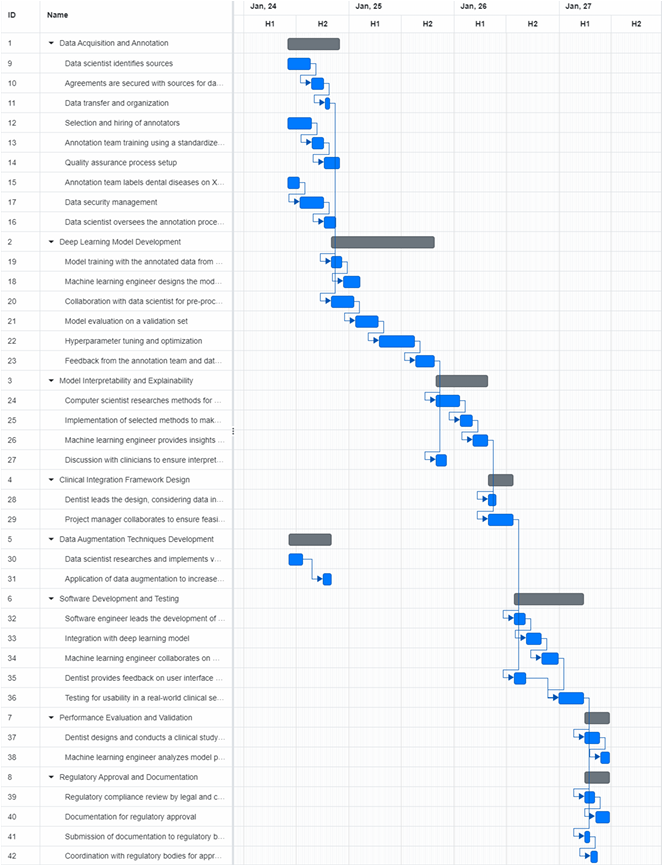
\includegraphics[width = 0.5\textwidth]{fig/tasks.png}
      \caption{Coordination and task schedule}
  \end{figure}
  
  \end{frame}

\section{Bibliography}

\begin{frame}[allowframebreaks]{Bibliography}

\setbeamertemplate{bibliography item}{\insertbiblabel}
\bibliographystyle{unsrt}
\bibliography{reference}

\end{frame}

\end{document}
